\documentclass[9pt]{beamer}

\mode<presentation> {

\usetheme{Madrid}

\usepackage{amsfonts}
\usepackage{mathrsfs}
\usepackage{amscd}
\usepackage{amsmath}
\usepackage{amssymb}
\usepackage{latexsym}
\usepackage{lscape}
\usepackage{xypic}
\usepackage{comment}
\usepackage{amscd}
\usepackage{wasysym}  
\usepackage{tikz}
\usetikzlibrary{cd, external, decorations.pathmorphing, fit, backgrounds, tikzmark, calc, shapes.misc, positioning}

\usepackage{tabularx}

\usepackage{appendix}
\usepackage{geometry}
\usepackage[nice]{nicefrac}
\usepackage{dsfont, stmaryrd}
\usepackage{array}

\usepackage{listings}
\usepackage{lstautogobble}
\usepackage{lstlinebgrd}

\usepackage{bbm}
\usepackage{xcolor}
\definecolor{keywordcolor}{rgb}{0.7, 0.1, 0.1}   % red
\definecolor{tacticcolor}{rgb}{0.0, 0.1, 0.6}    % blue
\definecolor{commentcolor}{rgb}{0.4, 0.4, 0.4}   % grey
\definecolor{symbolcolor}{rgb}{0.0, 0.1, 0.6}    % blue
\definecolor{sortcolor}{rgb}{0.1, 0.5, 0.1}      % green
\definecolor{attributecolor}{rgb}{0.7, 0.1, 0.1} % red
\def\lstlanguagefiles{lstlean.tex}
% set default language
\lstset{
  language=lean, 
  basicstyle=\ttfamily,
  autogobble=true,
  escapeinside={(*@}{@*)},
  captionpos=t,
  aboveskip=0.5em,
  belowskip=0.5em}

\usepackage{mymacros}
\usepackage{soul}
\usepackage[most]{tcolorbox}
\tcbuselibrary{theorems, skins, breakable}
% \usepackage{MnSymbol}
\usepackage{upgreek}

\newcommand{\nc}{\newcommand}
\newtheorem{prop}[theorem]{Proposition}

\newtheorem{theo}[theorem]{Theorem}

\newtheorem{coro}[theorem]{Corollary}

\newtheorem{defi}[theorem]{Definition}


\newtheorem{exam}[theorem]{Example}


\nc{\Spec}{{{\mathrm{Spec}}}}
\nc{\Hom}{{{\mathrm{Hom}}}}
\nc{\homm}{{\underline{\mathrm{Hom}}}}
\nc{\frakg}{{\mathfrak{g}}}
\nc{\fm}{{\mathfrak{m}}}
\nc{\fa}{{\mathfrak{a}}}
\nc{\calA}{{\mathcal A}}
\nc{\calB}{{\mathcal B}}
\nc{\calC}{{\mathcal C}}
\nc{\calD}{{\mathcal D}}
\nc{\calE}{{\mathcal E}}
\nc{\calF}{{\mathcal F}}
\nc{\calG}{{\mathcal G}}
\nc{\calH}{{\mathcal H}}
\nc{\calI}{{\mathcal I}}
\nc{\calJ}{{\mathcal J}}
\nc{\calK}{{\mathcal K}}
\nc{\calL}{{\mathcal L}}
\nc{\calM}{{\mathcal M}}
\nc{\calN}{{\mathcal N}}
\nc{\calO}{{\mathcal O}}
\nc{\calP}{{\mathcal P}} 
\nc{\calQ}{{\mathcal Q}} 
\nc{\Q}{{\mathbb Q}}
\nc{\R}{{\mathbb R}}
\nc{\calS}{{\mathcal S}}
\nc{\calT}{{\mathcal T}}
\nc{\calU}{{\mathcal U}}
\nc{\calV}{{\mathcal V}}
\nc{\calW}{{\mathcal W}}
\nc{\calX}{{\mathcal X}}
\nc{\calY}{{\mathcal Y}}

\nc{\bbZ}{{\mathbb{Z}}}
\nc{\zp}{{\mathbb{Z}_p}}

\nc{\bbN}{{\mathbb{N}}}

\nc{\fp}{{\mathfrak{p}}}

\nc{\fq}{{\mathfrak{q}}}


\nc{\proj}{{\mathrm{Proj}}}


\nc{\N}{{\mathbb{N}}}

\nc{\bbP}{{\mathbb{P}}}
\nc{\Z}{{\mathbb{Z}}}
\nc{\C}{{\mathbb{C}}}
\nc{\Gm}{{\mathbb{G}_m}}
\nc{\Aa}{{\mathbb{A}}}


%\setbeamertemplate{footline} % To remove the footer line in all slides uncomment this line
%\setbeamertemplate{footline}[page number] % To replace the footer line in all slides with a simple slide count uncomment this line

%\setbeamertemplate{navigation symbols}{} % To remove the navigation symbols from the bottom of all slides uncomment this line
}
\usepackage{tikz}
\usetikzlibrary{calc}
\usepackage{graphicx} % Allows including images
\usepackage{booktabs} % Allows the use of \toprule, \midrule and \bottomrule in tables

%----------------------------------------------------------------------------------------
%	TITLE PAGE
%----------------------------------------------------------------------------------------

\title[ Proj and Formalisation]{$~~~~$ Formalising the Multigraded Proj Construction in Lean 4. $~~~~$\\ }

\author{Arnaud Mayeux and Jujian Zhang } 
\institute[] 
{
\\ 
\medskip
\textit{} 
}
\date{Formalisation of mathematics with interactive theorem provers  \\ Thursday 19 June 2025 } 

\begin{document}

\begin{frame}
\titlepage % Print the title page as the first slide


\end{frame}




\begin{frame}{Introduction}
Inspired by projective geometry, Grothendieck defined the Proj scheme of a $\bbN$-graded ring $A$. This is a well-known construction that every mathematician in scheme theory knows and that is explained in most books about algebraic geometry. 


\[
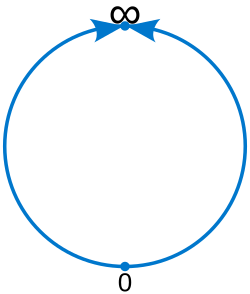
\includegraphics[scale=0.24]{p1.png} \]\[  \mathrm{Proj} (\mathbb{R}[X,Y])
\]
\[deg(X)=deg(Y)=1\]
\end{frame}
\begin{frame}


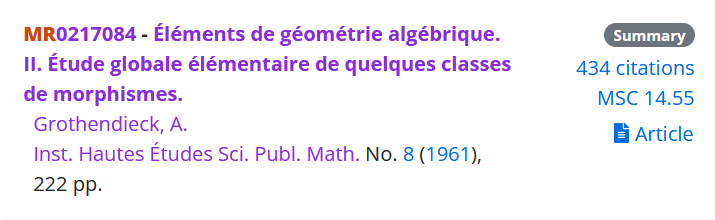
\includegraphics[scale=0.6]{EGA1961.png}

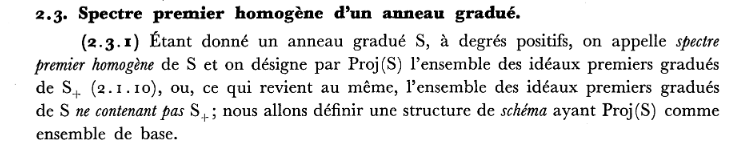
\includegraphics[scale=0.6]{captureEGA1961.png}

\end{frame}

\begin{frame}
In Hartshorne: 

\[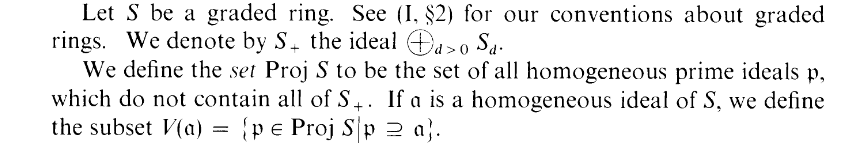
\includegraphics[scale=0.4]{captureHartshorne.png}\]

\[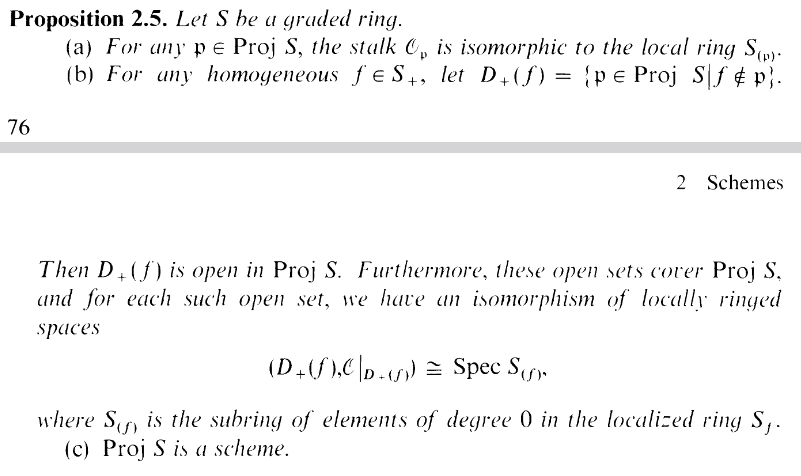
\includegraphics[scale=0.4]{captureHartshorne2.png}\]
\end{frame}
\begin{frame}
Similar treatments appear in:

$~~$

A. Ducros: "Introduction à la théorie des schémas" (Msc course 2021 Paris)

$~~$

R. Vakil : "THE RISING SEA Foundations of Algebraic Geometry" (Msc book course 2024 Stanford)

$~~$

Görtz-Wedhorn: "Algebraic Geometry I: Schemes " (Msc book course 2010)

$~~$

Eisenbud-Harris: "The geometry of schemes" (Msc book course 2000)


$~~$

Qing Liu: "Algebraic Geometry and Arithmetic Curves" (Msc book course 2002)

$~~$

Stacks Project 

$~~$


...



Beyond the definition of Proj, most of these treatments also study quasi-coherent sheaves and twisting sheaves on Proj and use Proj to define "blowups."  

This construction was formalised by J. Zhang in Lean. 

So it seems it is the end of this Proj story. 

But...
\end{frame}
 \begin{frame}
Question: Why Grothendieck assume that $A$ is $\bbN$-graded instead of graded by a general commutative monoid or group ? 

$~$

Answer: No reason from the point of view of Grothendieck scheme theory, in fact Brenner-Schröer defined the Proj of a ring graded by an arbitrary finitely generated abelian group $M$.

\[

\includegraphics[scale=0.5]{BS.png}\]\[
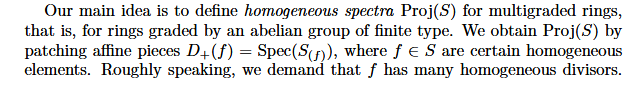
\includegraphics[scale=0.6]{captureBS.png}
\]
\end{frame}

\begin{frame}
None of the above references mention Brenner-Schröer work. 

$~~$

 In fact, versions of the multigraded Proj construction appear implicitly or
explicitly (but without reference to Brenner-Schröer) in various constructions in Geometric Representation Theory, including:

$~~$

P. Achar and L. Rider, The affine Grassmannian and the Springer resolution in positive characteristic, Compos. Math. 152 (2016), no. 12, 2627–2677. 

$~~$

S. Arkhipov and R. Bezrukavnikov, Perverse sheaves on affine flags and Langlands dual group,
with an appendix by R. Bezrukavnikov and I. Mirkovic, Israel J. Math. 170 (2009), 135–183.

$~~$

S. Arkhipov, R. Bezrukavnikov, and V. Ginzburg, Quantum groups, the loop Grassmannian,
and the Springer resolution J. Amer. Math. Soc. 17 (2004), no. 3, 595–678. 

$~~$

Goal of this talk: discuss Brenner-Schröer construction, new results and formalization. 
\end{frame}



\begin{frame}{References for this talk }

$~~$

H. Brenner and S. Schr\"oer, Ample families, multihomogeneous spectra, and algebraization of formal schemes, Pacific J. Math. {\bf 208} (2003), no.~2, 209--230.

\textbf{
(definition of multigraded Proj, separation, base change, ...)}

$~~$

A. Mayeux and S. Riche, On multi-graded Proj schemes, to appear in P.R.I.M.S., Kyoto University

\textbf{
(commutative algebra, twisting sheaves, functoriality, products, qcoh sheaves, ...)}

$~~$


A. Mayeux and J. Zhang, Multi-graded Proj construction in Lean4, https://github.com/ProjConstruction/Proj (2025)

\textbf{
(formalisation in Lean4, commutative algebra)}

$~~$

J. Zhang, Formalising the Proj construction in Lean, in {\it 14th International Conference on Interactive Theorem Proving}, Art. No. 35, LIPIcs. Leibniz Int. Proc. Inform., 268 (2023).

\textbf{
(formalisation in Lean4 of $\bbN$-graded Proj)}
\end{frame}


\begin{frame}{Why formalizing? }

Being sure that there is no error (rigor).

$~~$

$~~$

Provide data for future AI-mathematics.




\end{frame}


\begin{frame}{Graded localization}
If a given commutative ring $A$ is $M$-graded for some abelian group $M$, we will say that a multiplicative subset is homogeneous if it consists of homogeneous elements. 

If $A$ is a commutative $M$-graded ring and $S \subset A$ is a homogeneous multiplicative subset, the localization $A_S$ of $A$ with respect to $S$ is canonically $M$-graded, explicitly, for $m \in M$ we have
\[
( A_S)_m =  \left\{ \frac{a}{s} : \exists m', m'' \in M \text{ such that }  a \in A_{m'}, \, s \in (S \cap A_{m''}) \text{ and
$m'-m'' =m$ }\right\}.
%\subset A_S.
\]


Given a graded $A$-module $Q$, one can also consider the associated localization $Q_S$, which has a natural structure of a graded $A_S$-module.

\end{frame}

\begin{frame}

Given a homogeneous multiplicative subset $S \subset A$, we will denote by $\underline{S}$ the homogeneous multiplicative subset consisting of homogeneous divisors of elements in $S$. Note that we have a canonical isomorphism of graded rings
\begin{equation}
\label{eqn:isom-localizations}
 A_{ \underline{S}} \cong A_{S}.
\end{equation}
If $Q$ is a graded $A$-module we also have a canonical identification of graded abelian groups 
\begin{equation}
\label{eqn:isom-localizations-modules}
Q_{\underline{S}} \cong Q_S
\end{equation}
compatible with the actions of $A_{ \underline{S}} = A_{S}$.

\end{frame}


\begin{frame}


Consider an abelian group $M$, and a commutative $M$-graded ring $A$. 

 \begin{block}{Definition}
 Let $S$ be a homogeneous subset of $A$. We denote by $\deg(S)$ the subset of $M$ defined as 
\[\deg(S):= \{ m \in M : \exists s \in S , s  \in A_m \}. \]
 \end{block} 
Note that $\deg(\{0\})=M$.
More generally, if $S$ is a homogeneous multiplicative subset of $A$, then $\deg(S)$ is a submonoid of $M$.

\begin{block}{Definition}
Let $S$ be a homogeneous multiplicative subset of $A$. 
 We put $M[S]= \langle \deg (S) \rangle $, the subgroup of $M$ generated by $\deg(S)$.

\end{block}


\begin{block}{Definition (Relevant)}
\begin{enumerate} \item 
 A homogeneous multiplicative subset $S$ of $A$ is called \emph{$M$-relevant} (or just \emph{relevant} if $M$ is clear from the context) if for any $m$ in $M$ there exists $n \in \bbZ_{> 0}$ such that $nm$ belongs to $M[\underline{S}]$, i.e. if $M/(M[\underline{S}])$ is a torsion abelian group.

 \item
 A family $\{a_i : i \in I\}$ of homogeneous elements in $A$ is called $M$-relevant if the multiplicative subset generated by the $a_i$'s is relevant.
 \item
 A homogeneous element $a \in A$ is called $M$-relevant if the family $\{a\}$ is $M$-relevant.
\end{enumerate}\end{block}

\end{frame}


\begin{frame}


Let $M$ be an abelian group, and let $A$ be a commutative $M$-graded ring.

Let $S$ be a homogeneous multiplicative subset of $A$. \begin{block}{Definition}
\begin{enumerate}
\item
The degree-$0$ part $(A_S)_0$ of the localization $A_{S}$ is denoted by $A_{(S)}$ and is called the \emph{potion} of $A$ with respect to $S$. 
\item
If $Q$ is a graded $A$-module, we will also denote by $Q_{(S)}$ the degree-$0$ part $(Q_S)_0$ of $Q_S$; it admits a canonical structure of an $A_{(S)}$-module.
\end{enumerate}
\end{block}


We have canonical identifications
$A_{(\underline{S})} \cong A_{(S)}$ and $Q_{(\underline{S})} \cong Q_{(S)}$.


If $S$ and $T$ are multiplicative subsets of $A$, we will denote by $ST$ the multiplicative subset of $A$ generated by $S \cup T$, i.e. $ST = \{st : s \in S, \, t \in T \}$. Of course, $ST$ is homogeneous if $S$ and $T$ are.\end{frame}\begin{frame}
The following is the key result that makes the Proj construction work.

\begin{block}{Proposition (Magic of potions)}
\label{prop:magical} 
Let $S$ and $T$ be homogeneous multiplicative subsets of $A$. 
\begin{enumerate}
\item 
\label{it:magic-1}
We have a canonical homomorphism of potion rings 

$A_{(S )} \to  A_{(ST )}$.
%\]
\item 
\label{it:magic-2}
Assume that $S$ is relevant. Fix a subset $T' \subset T$ which generates $T$ as a submonoid of $(A,\times)$ and, for any $t $ in $T'$, fix $n_t \in \mathbb{N}_{>0}$ and $s_t, s_t' \in \underline{S}$ such that $\deg(t^{n_t}) = \deg(s_t)-\deg(s_t')$.
%$t^{n_t} \smile s_t$. 
Then $\frac{t^{n_t} s_t'} { s_t}$ belongs to $A_{(\underline{S} )}=A_{(S)}$. 
 Moreover we have a canonical isomorphism of $A_{(S )}$-algebras between $ A_{(ST )}$ and the localization of $A_{(S )}$ with respect to the multiplicative subset of $A_{(S)}$ generated by $\{\frac{t^{n_t} s_t'} { s_t} : t \in T' \}$.
\item 
\label{it:magic-3}
Assume that $S$ is relevant and that $T$ is finitely generated as submonoid of $(A,\times)$. The morphism of schemes 
$
\mathrm{Spec} (A_{(ST )}) \to \mathrm{Spec} (A_{(S)})
$
induced by the ring homomorphism in~\eqref{it:magic-1} is an open immersion of schemes.
\item 
\label{it:magic-4}
Let $f_1, \ldots, f_n \in A$ be nonzero relevant homogeneous elements of the same degree.
Then we have a canonical open immersion
\[
\Spec(A_{ (f_1 + \cdots + f_n) }) \to \Spec (A_{(f_1)}) \cup \cdots \cup \Spec (A_{(f_n)})
\]
where the right-hand side is defined as the glueing of the affine schemes $\Spec (A_{(f_i)})$ along the open subschemes $\Spec (A_{(f_i \cdot f_j)}) \subset \Spec (A_{(f_i)})$ (see~\eqref{it:magic-3}).

\end{enumerate}
\end{block}
\end{frame}

\begin{frame}


From now on we assume that $M$ is a \emph{finitely generated} abelian group, and fix a commutative $M$-graded ring $A$.

We will denote by $\mathcal{F}_A$ the set of all relevant homogeneous multiplicative subsets of $A$ which are finitely generated as submonoids of $(A,\times)$ ("good potion ingredients").

\begin{block}{Construction (Proj as glueing potions)}

Let
$\mathcal{F} \subset \mathcal{F}_A$ be a subset.
 For each $S \in \mathcal{F}$, let $D_{\dagger}(S)$ be the spectrum of the potion $A_{(S)}$. 
 If $S,T \in \mathcal{F}$, the affine scheme $D_{\dagger}(ST)$ identifies canonically with an open subscheme of $D_{\dagger}(S)$. For each $S,T \in \mathcal{F}$, we have equalities
 \[
 D_{\dagger}({S S}) = D_{\dagger}(S) \quad \text{and} \quad D_{\dagger}({ST})=D_{\dagger}({TS}).
 \]
 Moreover, for each triple $S,T,U \in \mathcal{F}$, we have
 \[
 D_{\dagger}({ST} )\cap D_{\dagger}({SU}) = D_{\dagger}({TS}) \cap D_{\dagger}({TU}).
 \]

Now, by glueing, from these data we obtain a scheme $\mathrm{Proj}^M_{\mathcal{F} } (A)$ and, for each $S \in \mathcal{F}$, an open immersion $\varphi_S : D_{\dagger}(S) \to \mathrm{Proj}^M_{\mathcal{F}} (A)$, such that
\[
\mathrm{Proj}^M_{\mathcal{F} } (A) = \bigcup_{S \in \mathcal{F} } \varphi_S( D_{\dagger}(S)).
\]

In practice, we will often identify $D_{\dagger}(S) $ and $\varphi_S (D_{\dagger}(S))$. 


In the case when $\mathcal{F} = \mathcal{F}_A$,
 the scheme $\mathrm{Proj}^M_{\mathcal{F}_A} (A)$ will be denoted $\mathrm{Proj}^M(A)$, or just $\mathrm{Proj}( A)$ when $M$ is clear from the context.
 \end{block}

 \end{frame}




\begin{frame}

\begin{block}{Proposition} 
The scheme $\mathrm{Proj}^M(A)$ is quasi-separated.
\end{block}

\begin{block}{Proposition (Functoriality of Proj)} 
Let $\Psi:A \to B $ be a homomorphism of $M$-graded rings. 
For any $\mathcal{F} \subset \mathcal{F}_A$ 
we have a canonical morphism of schemes $\mathrm{Proj}^M_{\Psi (\mathcal{F})} (B) \to \mathrm{Proj}^M_{\mathcal{F} } (A)$. Moreover, for any $S \in \calF$ we have
\begin{equation}
\mathrm{Proj}^M_{\Psi(\calF)}(B) \times_{\mathrm{Proj}_{\calF}^M(A)} D_\dag(S) = D_\dag(\Psi(S));
\end{equation}
in particular, the morphism is affine.
\end{block}

\begin{block}{Proposition}
Assume that $\Psi : A \to B$ is surjective. Then we have $\mathrm{Proj}^M_{\Psi (\mathcal{F}_A)} (B) = \mathrm{Proj}^M (B)$, and the canonical morphism
 $\mathrm{Proj}^M(B) \to \mathrm{Proj}^M(A)$
is a closed immersion.
\end{block}

 \end{frame}


\begin{frame}

\begin{block}{Proposition}
 Let $M$ and $M'$ be two finitely generated abelian groups. Let $R$ be a commutative ring and let $A$ (resp.~$A'$) be a commutative $M$-graded (resp.~$M'$-graded) $R$-algebra. 
 Then for the natural $(M \times M')$-grading on $A \otimes_R A'$, we have a canonical isomorphism
 \[
 \mathrm{Proj} ^{M \times M'} (A \otimes_R A') \cong \mathrm{Proj} ^M (A) \times_{\Spec(R)} \mathrm{Proj} ^{M'} (A'). 
 \]
\end{block}

\end{frame}



\begin{frame}{Quasi-coherent sheaves}

Let $Q$ be an $M$-graded $A$-module. For any homogeneous multiplicative subset $S \subset A$, we have considered the $A_{(S)}$-module $Q_{(S)}$. The following fact is immediate by glueing of quasi-coherent sheaves.


\begin{block}{Definition}
There exists 
a unique quasi-coherent $\mathcal{O}_{\mathrm{Proj}^M(A)}$-module $\widetilde{Q}$ such that
$\Gamma \bigl( D_\dag(S)  , \widetilde{Q} \bigr) = Q_{(S)}$
for every $S \in \calF_A$.
\end{block}

An $M$-graded $A$-module $Q$ will be called \emph{negligible} if $\widetilde{Q}=0$.


\end{frame}


\begin{frame}{Twisting sheaves}

If $Q$ is a graded $A$-module and $\alpha \in M$, we will denote by $Q(\alpha)$ the $M$-graded $A$-module which coincides with $M$ as an $A$-module, but with the $M$-grading defined by $(Q(\alpha))_\beta = Q_{\alpha+\beta}$ for $\beta \in M$.


\begin{block}{Definition (Twisting sheaves)}
Let $\alpha \in M$.
\begin{enumerate}
\item
The quasi-coherent sheaf $\widetilde{A(\alpha)}$ on $\mathrm{Proj}^M(A)$ is 
denoted $\mathcal{O}_{\mathrm{Proj}^M(A)} (\alpha)$.
\item
If $\calQ$ is a sheaf of $\calO_{\mathrm{Proj}^M(A)}$-modules, we set $\calQ (\alpha) = \calO_{\mathrm{Proj}^M(A)} (\alpha ) \otimes_{\calO_{\mathrm{Proj}^M(A)}} \calQ$.
\end{enumerate}
\end{block}


\begin{block}{Proposition}
Assume that $A$ is a noetherian ring.
\begin{enumerate}
\item
For any $\alpha \in M$, the quasi-coherent sheaf $\mathcal{O}_{\mathrm{Proj}^M(A)} (\alpha)$ is coherent.
\item
If $Q$ is a finitely generated $M$-graded $A$-module, then $\widetilde{Q}$ is coherent.
\end{enumerate}
\end{block}


\end{frame}

\begin{frame}

A family $S \in \calF_A$ will be called \emph{maximally relevant} if $M[\underline{S}]=M$.   We will denote by $\calF_A^{\mathrm{m}} \subset \calF_A$ the subset consisting of maximally relevant families. We explore various consequences of the following condition :
\begin{equation}
\label{eqn:cover-max}
\mathrm{Proj}^M(A) = \bigcup_{S \in \calF_A^{\mathrm{m}}} D_\dag(S).
\end{equation}


\begin{block}{Proposition}
Assume that~\eqref{eqn:cover-max} is satisfied. Then for any $ \alpha \in M$, the quasi-coherent $\calO_{\mathrm{Proj}^M(A)}$-module $\calO_{\mathrm{Proj}^M(A)} (\alpha)$ is an invertible sheaf.
\end{block}

\begin{block}{Proposition}
Assume that~\eqref{eqn:cover-max} is satisfied, and moreover that $\mathrm{Proj}^M(A)$ is quasi-compact. Then the functor
\[
\mathsf{L} : \mathrm{Mod}^M(A) / \mathrm{Mod}^M(A)_{\mathrm{neg}} \to \mathrm{QCoh}(\mathrm{Proj}^M(A))
\]
is an equivalence of categories.
\end{block}
\end{frame}



\begin{frame}{Example: Flag variety as Proj}
 Let $k$ be an algebraically closed field and let $G$ be
a connected reductive group scheme over $k.$ Let $T$ be a maximal split torus
and $B$ be a Borel subgroup such that $B = T N$ where $N$ is the unipotent
radical. Then $G/N$ is quasi-affine and the ring $A := \Gamma (G/N, \mathcal{O}_{G/N} )$ is canonically $X^*(T)$-graded. 

\begin{block}{Proposition}
The flag variety $G/B$ identifies with $\mathrm{Proj}^{X^*(T)} (A)$.
\end{block}
Consider a finite-dimensional $G$-module $\widetilde{V}$ and a $B$-stable subspace $V \subset \widetilde{V}$. 
We can then consider the induced scheme
\[
 G \times^{B} V,
\]
i.e.~the quotient of the product $G \times V$ by the (free) action of $B$ defined by $b \cdot (g,x) = (gb^{-1}, b \cdot x)$.  It is a vector bundle over $G/B$.

There is a canonical way to see such schemes as Proj schemes.

An interesting case is the \emph{Springer resolution}.

\end{frame}


\begin{frame}{Comparison}


\begin{tabular}{|l|c|r|}
  \hline
  \textbf{Property of the Proj construction} & Grothendieck setting  & Brenner-Schröer setting \\
  \hline
  Grading & $\bbN $ & \text{any f.g. ab. gp $M$} \\
  \hline
  Definition via prime ideals works & Yes & No\\
   \hline
  Definition via prime ideals required & No & No\\
  \hline
  Definition via glueing works & Yes & Yes\\
  \hline 
  Glueing steps required & Yes & Yes \\ 
  \hline
  Twsiting sheaves available & Yes & Yes \\ 
  \hline
 Compatible with tensor product & No & Yes \\ 
  \hline
  Separated & Yes & No, but quasi-separated \\
  \hline 
  Compatible with blowups & Yes & Yes \\
  \hline 
  Allows to describe G/B canonically  & No & Yes \\
  \hline 
  Qcoh on Proj via graded modules   & Yes & Yes \\
  \hline 
  Verified in Lean    & Yes & Yes \\
  \hline 
\end{tabular}

$~~$

$~~$

Moreover: 

The level of technicality in the Grothendieck setting is almost the same as that in the Brenner–Schröer setting.

\end{frame}



\begin{frame}{Lean4 Formalization}

In our joint work on the formalization we formalized: 
\begin{enumerate}
\item Localization of graded rings and potions

\item Magic of potions 

\item The definition of Proj via glueing 

\item Twisting modules
\end{enumerate}
We plan to formalize:

\begin{enumerate} \item Existence of blowups via Proj and dilatations 
\item Quasi-coherent sheaves on Proj
\end{enumerate}



We use much of the material on the formalization of scheme theory available in mathlib (Buzzard et al.).
Previously, Jujian Zhang formalized the $\mathbb{N}$-graded $\mathrm{Proj}$ construction, and we use a lot of graded algebras from this work. 



 Though the multi-graded Proj construction generalises the $\mathbb{N}$-graded one, the formalisations remain independent because we used the gluing approach instead of the graded ideals approach. 


\end{frame}




\begin{frame}{Various remarks}
\begin{itemize}

\item Collaborating was very useful as we had complementary backgrounds.
  
\item In the long run, we expect formalised mathematics to become more and more popular. Formalised mathematics is required for rigorous (non-hallucinating) AI-generated advanced mathematical research.  
  
\item It would be very nice to see advances in AI-automated formalisation and a more \LaTeX-friendly interface for formalisation.
  
\item As of Spring 2025, Copilot (Lean AI) remained sometimes helpful but insufficiently effective for assisting with the formalisation of algebraic geometry. Copilot was not able to prove that $0 \times 1 = 0$ in a certain non-trivial graded ring.

\end{itemize}


\end{frame}


\section{Implementation in Lean4}
\begin{frame}[fragile]
\frametitle{Graded objects in Lean4}

\begin{lstlisting}[mathescape=true, extendedchars=true]
variable {A M ιA ιM σA σM : Type*} 
variable [Ring A] [AddCommGroup M] [Module A M]
variable ($\mathcal{A}$ : ιA → σA) ($\mathcal{M}$ : ιM → σM)
variable [DecidableEq ιA] [AddMonoid ιA] [DecidableEq ιM]  [VAdd ιA ιM]
variable [SetLike σA A] [SetLike σM M]
variable [AddSubgroupClass σA A] [AddSubgroupClass σM M] 
variable [GradedRing $\mathcal{A}$] 
variable [DirectSum.Decomposition $\mathcal{M}$] [SetLike.GradedSMul $\mathcal{A}$ $\mathcal{M}$]
\end{lstlisting}
\begin{itemize}
  \item \lstinline|[SetLike σA A]| and \lstinline|[AddSubgroupClass σA A]| together assert that the terms of \lstinline|σA| are subgroups of $A$.
%   \item<2> \lstinline[mathescape=true]|[GradedRing $\mathcal{A}$]| is an abbreviation for \lstinline[mathescape=true]|[DirectSum.Decomposition $\mathcal{A}$]| and 
% \lstinline[mathescape=true]|[SetLike.GradedMonoid $\mathcal{A}$]| where \lstinline[mathescape=true]|[SetLike.GradedMonoid $\mathcal{\McA}$]| is an abbreviation for 
% \lstinline[mathescape=true]|[SetLike.GradedOne $\mcA$]| asserting that $1$ has grade zero and \lstinline[mathescape=true]|[SetLike.GradedMul $\mcA$]| asserting that $\mcA_i\mcA_j \subseteq \mcA_{i+j}$.
%   \item<3> \lstinline[mathescape=true]|[SetLike.GradedSMul $\mcA$ $\mcM$]| asserts that $\mcA_i \cdot \mcM_j \subseteq \mcM_{i+j}$ where $i + j$ is provided by \lstinline|[VAdd ιA ιM]|. 
%   \item<4> The general setup here is versatile: by allowing \lstinline|ιA| and \lstinline|ιM| to be different types, we can have graded rings and modules that are not graded by the same monoid --- for example the ring is graded by $\NN$ and the module by $\ZZ$.
\end{itemize}
\end{frame}


\begin{frame}[fragile]
\frametitle{Graded objects in Lean4}

\begin{lstlisting}[mathescape=true, extendedchars=true]
variable {A M ιA ιM σA σM : Type*} 
variable [Ring A] [AddCommGroup M] [Module A M]
variable ($\mathcal{A}$ : ιA → σA) ($\mathcal{M}$ : ιM → σM)
variable [DecidableEq ιA] [AddMonoid ιA] [DecidableEq ιM]  [VAdd ιA ιM]
variable [SetLike σA A] [SetLike σM M]
variable [AddSubgroupClass σA A] [AddSubgroupClass σM M] 
variable [GradedRing $\mathcal{A}$] 
variable [DirectSum.Decomposition $\mathcal{M}$] [SetLike.GradedSMul $\mathcal{A}$ $\mathcal{M}$]
\end{lstlisting}
\begin{itemize}
  % \item<1> \lstinline|[SetLike σA A]| and \lstinline|[AddSubgroupClass σA A]| together assert that the terms of \lstinline|σA| are subgroups of $A$.
  \item\lstinline[mathescape=true]|[GradedRing $\mathcal{A}$]| is an abbreviation for \lstinline[mathescape=true]|[DirectSum.Decomposition $\mathcal{A}$]| and 
\lstinline[mathescape=true]|[SetLike.GradedMonoid $\mathcal{A}$]| where \lstinline[mathescape=true]|[SetLike.GradedMonoid $\mathcal{\McA}$]| is an abbreviation for 
\lstinline[mathescape=true]|[SetLike.GradedOne $\mcA$]| asserting that $1$ has grade zero and \lstinline[mathescape=true]|[SetLike.GradedMul $\mcA$]| asserting that $\mcA_i\mcA_j \subseteq \mcA_{i+j}$.
  % \item<3> \lstinline[mathescape=true]|[SetLike.GradedSMul $\mcA$ $\mcM$]| asserts that $\mcA_i \cdot \mcM_j \subseteq \mcM_{i+j}$ where $i + j$ is provided by \lstinline|[VAdd ιA ιM]|. 
  % \item<4> The general setup here is versatile: by allowing \lstinline|ιA| and \lstinline|ιM| to be different types, we can have graded rings and modules that are not graded by the same monoid --- for example the ring is graded by $\NN$ and the module by $\ZZ$.
\end{itemize}
\end{frame}


\begin{frame}[fragile]
\frametitle{Graded objects in Lean4}

\begin{lstlisting}[mathescape=true, extendedchars=true]
variable {A M ιA ιM σA σM : Type*} 
variable [Ring A] [AddCommGroup M] [Module A M]
variable ($\mathcal{A}$ : ιA → σA) ($\mathcal{M}$ : ιM → σM)
variable [DecidableEq ιA] [AddMonoid ιA] [DecidableEq ιM]  [VAdd ιA ιM]
variable [SetLike σA A] [SetLike σM M]
variable [AddSubgroupClass σA A] [AddSubgroupClass σM M] 
variable [GradedRing $\mathcal{A}$] 
variable [DirectSum.Decomposition $\mathcal{M}$] [SetLike.GradedSMul $\mathcal{A}$ $\mathcal{M}$]
\end{lstlisting}
\begin{itemize}
%   \item<1> \lstinline|[SetLike σA A]| and \lstinline|[AddSubgroupClass σA A]| together assert that the terms of \lstinline|σA| are subgroups of $A$.
%   \item<2> \lstinline[mathescape=true]|[GradedRing $\mathcal{A}$]| is an abbreviation for \lstinline[mathescape=true]|[DirectSum.Decomposition $\mathcal{A}$]| and 
% \lstinline[mathescape=true]|[SetLike.GradedMonoid $\mathcal{A}$]| where \lstinline[mathescape=true]|[SetLike.GradedMonoid $\mathcal{\McA}$]| is an abbreviation for 
% \lstinline[mathescape=true]|[SetLike.GradedOne $\mcA$]| asserting that $1$ has grade zero and \lstinline[mathescape=true]|[SetLike.GradedMul $\mcA$]| asserting that $\mcA_i\mcA_j \subseteq \mcA_{i+j}$.
  \item \lstinline[mathescape=true]|[SetLike.GradedSMul $\mcA$ $\mcM$]| asserts that $\mcA_i \cdot \mcM_j \subseteq \mcM_{i+j}$ where $i + j$ is provided by \lstinline|[VAdd ιA ιM]|. 
  % \item The general setup here is versatile: by allowing \lstinline|ιA| and \lstinline|ιM| to be different types, we can have graded rings and modules that are not graded by the same monoid --- for example the ring is graded by $\NN$ and the module by $\ZZ$.
\end{itemize}
\end{frame}

\begin{frame}[fragile]
\frametitle{Graded objects in Lean4}

\begin{lstlisting}[mathescape=true, extendedchars=true]
variable {A M ιA ιM σA σM : Type*} 
variable [Ring A] [AddCommGroup M] [Module A M]
variable ($\mathcal{A}$ : ιA → σA) ($\mathcal{M}$ : ιM → σM)
variable [DecidableEq ιA] [AddMonoid ιA] [DecidableEq ιM]  [VAdd ιA ιM]
variable [SetLike σA A] [SetLike σM M]
variable [AddSubgroupClass σA A] [AddSubgroupClass σM M] 
variable [GradedRing $\mathcal{A}$] 
variable [DirectSum.Decomposition $\mathcal{M}$] [SetLike.GradedSMul $\mathcal{A}$ $\mathcal{M}$]
\end{lstlisting}
\begin{itemize}
%   \item<1> \lstinline|[SetLike σA A]| and \lstinline|[AddSubgroupClass σA A]| together assert that the terms of \lstinline|σA| are subgroups of $A$.
%   \item<2> \lstinline[mathescape=true]|[GradedRing $\mathcal{A}$]| is an abbreviation for \lstinline[mathescape=true]|[DirectSum.Decomposition $\mathcal{A}$]| and 
% \lstinline[mathescape=true]|[SetLike.GradedMonoid $\mathcal{A}$]| where \lstinline[mathescape=true]|[SetLike.GradedMonoid $\mathcal{\McA}$]| is an abbreviation for 
% \lstinline[mathescape=true]|[SetLike.GradedOne $\mcA$]| asserting that $1$ has grade zero and \lstinline[mathescape=true]|[SetLike.GradedMul $\mcA$]| asserting that $\mcA_i\mcA_j \subseteq \mcA_{i+j}$.
  % \item \lstinline[mathescape=true]|[SetLike.GradedSMul $\mcA$ $\mcM$]| asserts that $\mcA_i \cdot \mcM_j \subseteq \mcM_{i+j}$ where $i + j$ is provided by \lstinline|[VAdd ιA ιM]|. 
  \item The general setup here is versatile: by allowing \lstinline|ιA| and \lstinline|ιM| to be different types, we can have graded rings and modules that are not graded by the same monoid --- for example the ring is graded by $\NN$ and the module by $\ZZ$.
\end{itemize}
\end{frame}


\begin{frame}[fragile]
\frametitle{Graded Ring Homomorphisms}
\begin{lstlisting}[]
structure GradedRingHom extends RingHom A B where
  map_mem' : ∀ {i} {x : A}, 
    x ∈ 𝒜 i → toFun x ∈ ℬ i

scoped[Graded] infix:25 "→+*" => GradedRingHom
\end{lstlisting}

For a graded ring homomorphism $f : A \to B$, we define the corresponding ring homomorphism $\bigoplus_{i\in\iota}\mcA_i \to \bigoplus_{i\in\iota}\mcB_i$ by
\[
f_{\oplus} : \begin{tikzcd}[column sep=huge]
  \bigoplus_{i\in\iota} \mcA_i \arrow[r, "\decompose"] & A \arrow[r, "f"] & B \arrow[r, "\recompose"] & \bigoplus_{i\in\iota} \mcB_i.
\end{tikzcd}
\]
\begin{lstlisting}
def directSum (f : 𝒜 →+* ℬ) : (⨁ i, 𝒜 i) →+* (⨁ i, ℬ i) :=
  RingHom.comp (DirectSum.decomposeRingEquiv ℬ) <| 
    f.comp (DirectSum.decomposeRingEquiv 𝒜).symm
\end{lstlisting}

\end{frame}

% \begin{frame}[fragile]
%   \frametitle{Graded Ring Isomorphisms and Graded Algebra Homomorphisms etc.}
% \begin{lstlisting}[extendedchars=true]
% structure GradedRingEquiv extends RingEquiv A B where
%   map_mem' : ∀ {i : ι} {x : A}, x ∈ 𝒜 i → toFun x ∈ ℬ i
%   inv_mem' : ∀ {i : ι} {y : B}, y ∈ ℬ i → invFun y ∈ 𝒜 i

% scoped[Graded] infix:25 "≃+*" => GradedRingEquiv

% structure GradedAlgHom extends A →ₐ[R] B, GradedRingHom 𝒜 ℬ

% scoped[Graded] notation:25 𝒜 " →ₐ[" R "] " ℬ => 
%   GradedAlgHom (R := R) 𝒜 ℬ
% \end{lstlisting}
% \end{frame}


\begin{frame}[fragile]
  \frametitle{Localized Graded Rings}
  Let $S$ be a homogeneous submonoid of $A$. 
  Let $\mathcolorbox{yellow!10}{P_i}$ denote the set of qudraples $(a, b, d_a, d_b)$ where $d_a$ and $d_b$ are in $\iota$ such that $d_a - d_b = i$, 
$a \in A$ is homogeneous of degree $d_a$ and $b \in S$ is homogeneous of degree $d_b$.
For each $i \in \iota$, we give $P_i$ a group structure by: 
\begin{itemize}
  \item The zero element is $(0, 1, 0, 0)$.
  \item The result of adding $(a, b, d_a, d_b)$ and $(a', b', d_{a'}, d_{b'})$ is defined as
$(ab' + a'b, bb', d_a + d_{a'}, d_b + d_{b'})$.
  \item The negation of $(a, b, d_a, d_b)$ is defined as $(-a, b, d_a, d_b)$.
\end{itemize}
Hence, we have \sethlcolor{red!10}\hl{a group homomorphism $\mathsf{frac}: P_i \to A_{S}$ defined by $(a, b, d_a, d_{b}) \mapsto \frac{a}{b}$}.
Consider the quotient formed by $\quotient{P_{i}}{\sim}$ where \sethlcolor{green!10}\hl{two quadruples $p$ and $q$ are equivalent if and only if $\mathsf{frac}(p) = \mathsf{frac}(q)$}.
We take \sethlcolor{olive!10}\hl{the $i$-th grading $A_{S,i}$ of $A_S$ to be the range of the group homomorphism} \sethlcolor{purple!15}\hl{$\mathsf{frac} : \quotient{P_{i}}{\sim} \to A_{S}$}.

\end{frame}


\begin{frame}[fragile, allowframebreaks]
  \frametitle{Localized Graded Rings}
\begin{lstlisting}[linebackgroundcolor={%
  \ifnum\value{lstnumber}=10\color{red!10}\fi
  \ifnum\value{lstnumber}=11\color{red!10}\fi
  \ifnum\value{lstnumber}=12\color{red!10}\fi
  \ifnum\value{lstnumber}=13\color{red!10}\fi
  \ifnum\value{lstnumber}=14\color{red!10}\fi
  % \ifnum\value{lstnumber}=15\color{red!10}\fi
  \ifnum\value{lstnumber}=16\color{green!10}\fi
  \ifnum\value{lstnumber}=17\color{green!10}\fi
  % \ifnum\value{lstnumber}=19\color{green!10}\fi
  \ifnum\value{lstnumber}=19\color{purple!15}\fi
  \ifnum\value{lstnumber}=20\color{purple!15}\fi
  \ifnum\value{lstnumber}=21\color{purple!15}\fi
  % \ifnum\value{lstnumber}=24\color{purple!15}\fi
  \ifnum\value{lstnumber}=23\color{olive!10}\fi
  \ifnum\value{lstnumber}=24\color{olive!10}\fi
  \ifnum\value{lstnumber}=25\color{olive!10}\fi
}, caption={Grading of localized rings}]
structure (*@\sethlcolor{yellow!10}\hl{PreLocalizationGrading}@*) (i : ι) where
  num : A
  den : S.toSubmonoid
  degNum : ι
  degDen : ι
  num_mem : num ∈ 𝒜 degNum
  den_mem : (den : A) ∈ 𝒜 degDen
  deg_frac_eq : degNum - degDen = i

def val (i : ι) : 
    (S.PreLocalizationGrading i) →+ Localization S.toSubmonoid where
  toFun x := Localization.mk x.num x.den
  map_zero' := Localization.mk_zero 1
  map_add' := by simp [Localization.add_mk]

def addCon (i : ι) : AddCon (S.PreLocalizationGrading i) := 
  AddCon.ker (val S i)

def emb (i : ι) : 
    (addCon S i).Quotient →+ Localization S.toSubmonoid :=
  AddCon.lift _ (val ..) le_rfl

def LocalizationGrading (i : ι) : 
    AddSubgroup (Localization S.toSubmonoid) := 
  (PreLocalizationGrading.emb S i).range
\end{lstlisting} 
\end{frame}

\begin{frame}[fragile]
  \frametitle{Homogeneous Localization}
\begin{itemize}

  \item Let $R$ be a commutative ring and $A$ a commutative graded $R$-algebra. Let $x$ be a submonoid of $A$. 
  \item In general, unless $x$ contains only homogeneous elements, the localized ring $A_x$ is not graded.
  \item However, we can still investigate set $A_{(x)}$ of elements of degree zero in the localized ring. 
\end{itemize}

Consider the type $\mathcolorbox{yellow!10}{P}$ of triples of $(i, a, b)$ where $a$ and $b$ are 
  homogeneous elements of the degree $i$ and $b$ is in $x$, we have a function $\mathcolorbox{blue!10}{\mathsf{frac} : P \to A_{x}}$ defined by
  $(i, a, b) \mapsto =\frac a b$.
  We define the homogeneous localization $A_{(x)}$ to be the quotient $\quotient{P}{\sim}$ where \sethlcolor{red!10}\hl{two pairs $p$ and $q$
  are equivalent if and only if $\mathsf{frac}(p) = \mathsf{frac}(q)$}. 
  The function $\mathsf{frac}$ descends to an embedding $\mathcolorbox{green!10}{\iota: \hloca A{\mfp} \hookrightarrow A_{\mfp}}$.
\end{frame}

\begin{frame}[fragile]
  \frametitle{Homogeneous Localization}
\begin{lstlisting}[linebackgroundcolor={%
  \ifnum\value{lstnumber}=1\color{yellow!10}\fi
  \ifnum\value{lstnumber}=2\color{yellow!10}\fi
  \ifnum\value{lstnumber}=3\color{yellow!10}\fi
  \ifnum\value{lstnumber}=4\color{yellow!10}\fi
  \ifnum\value{lstnumber}=6\color{blue!10}\fi
  \ifnum\value{lstnumber}=7\color{blue!10}\fi
  \ifnum\value{lstnumber}=8\color{blue!10}\fi
  \ifnum\value{lstnumber}=13\color{green!10}\fi
  \ifnum\value{lstnumber}=14\color{green!10}\fi
  \ifnum\value{lstnumber}=15\color{green!10}\fi},
  mathescape=true, caption={Homogeneous Localization}]
structure NumDenSameDeg where
  deg : ι
  (num den : 𝒜 deg)
  den_mem : (den : A) ∈ x

def embedding (p : NumDenSameDeg 𝒜 x) : 
    Localization x :=
  Localization.mk p.num ⟨p.den, p.den_mem⟩

def HomogeneousLocalization : Type _ :=
  Quotient <| (*@\sethlcolor{red!10}\hl{Setoid.ker <| embedding $\mcA$ x}@*)

def val (y : HomogeneousLocalization 𝒜 x) : 
    Localization x :=
  Quotient.liftOn' y (embedding 𝒜 x) ...
\end{lstlisting}

Why not just use a subring of $A_x$? 
\end{frame}


% \begin{frame}[fragile]
%   \frametitle{Graded Tensor Products}
% \begin{itemize}
%   \item 
%   Let $A$ and $B$ be graded $R$-algebras where $A$ is graded by $\iota_{A}$ and $B$ is graded by $\iota_B$.
%   \item 
%   For any $i \in \iota_A$ and $j \in \iota_B$, the $(i,j)$-th graded piece of the tensor product $A \ox_R B$ is the 
%   $A_i \ox_R B_j$. 
%   \item 
%   Since type theoretically, we need $A_i \ox_R B_j$ as a submodule of $A \ox_R B$, we use the range 
%   of the linear map $A_i \ox_R B_j \to A \ox_R B$.
% \end{itemize}
%   \begin{lstlisting}[caption={Graded Tensor Product}]
% noncomputable def gradingByProduct : 
%     ιA × ιB → Submodule R (A ⊗[R] B) := fun p ↦ 
%   LinearMap.range (TensorProduct.map (𝒜 p.1).subtype (ℬ p.2).subtype)

% scoped infix:min "⊗" => gradingByProduct
%   \end{lstlisting}
% \end{frame}


\begin{frame}[fragile]
  \frametitle{Potions}
\begin{itemize}
  \item<1-> 
  Let $A$ be a commutative $R_0$-algebra that is graded by an abelian group $\iota$. 
  \item For any homogeneous submonoid $S \subseteq A$, we define the potion $\potion(S)$ to be the 
  homogeneous localization $\hloc A S$.
  \item<2-> If $\phi : A \to B$ is a graded ring homomorphism there is a ring homomorphism
  $\leanmath{potionToMap}: \potion(S) \to \potion\left(\phi_{\star} S\right)$ induced by $\phi$.
  \item<3-> If $S = T$ are two homogeneous submonoids of $A$, we have a ring isomorphism $\leanmath{potionEquiv}: \potion(S) \cong \potion(T)$.
  % In particular, since $S S = S$, we have a ring isomorphism $\potion(S)\cong \potion(SS)$.
  \item<4-> There is a ring homomorphism $\leanmath{potionToMul}:\potion(S) \to \potion(ST)$,
  with this ring homomorphism $\leanmath{potionToMul}$, we view $\potion(ST)$ as a $\potion(S)$-algebra.
  \item<5-> There is a ring isomorphism $\leanmath{equivBarPotion}: \potion(S) \cong \potion\left( \mybar{S} \right)$ induced by $\id_A$. This is \cref{eqn:isom-localizations} restricted to the zeroth degree.
\end{itemize}

\end{frame}

\begin{frame}[fragile]
  \frametitle{Potion Generator}
  Suppose $S$ and $T$ be homogeneous submonoids of $A$. A \emph{potion generator} of $T$ over $S$ is the following data:
\begin{itemize}
  \item \sethlcolor{yellow!10}\hl{an indexing set $I$};
  \item \sethlcolor{red!10}\hl{a family of elements $\left\{ t_i \middle| i \in I \right\} \subseteq T$ generating $T$ as submonoid};
  \item \sethlcolor{blue!10}\hl{two families of elements $\left\{ s_i \middle| i \in I \right\} \subseteq \mybar{S}$ and  
  $\left\{ s_i' \middle| i \in I \right\} \subseteq \mybar{S}$ such that each $s_j$ is homogeneous of degree $i_j$ and 
  each $s_j'$ is homogeneous of degree $i'_j$};
  \item \sethlcolor{green!10}\hl{a family of positive natural numbers $\left\{ n_i\middle| i\in I \right\}$, such that for each $j \in I$,
  $t_j^{n_j}$ is homogeneous of degree $i_j - i'_j$}.
\end{itemize}
  
\begin{lstlisting}[extendedchars=true, caption={Potion Generator}, 
  linebackgroundcolor={%
  \ifnum\value{lstnumber}=2\color{yellow!10}\fi
  \ifnum\value{lstnumber}=3\color{red!10}\fi
  \ifnum\value{lstnumber}=4\color{red!10}\fi
  \ifnum\value{lstnumber}=5\color{red!10}\fi
  \ifnum\value{lstnumber}=6\color{blue!10}\fi
  \ifnum\value{lstnumber}=7\color{blue!10}\fi
  \ifnum\value{lstnumber}=8\color{blue!10}\fi
  \ifnum\value{lstnumber}=9\color{blue!10}\fi
  \ifnum\value{lstnumber}=10\color{blue!10}\fi
  \ifnum\value{lstnumber}=11\color{blue!10}\fi
  \ifnum\value{lstnumber}=12\color{green!10}\fi
  \ifnum\value{lstnumber}=13\color{green!10}\fi}, linebackgroundsep=-8pt, linebackgroundwidth=280pt,
  basicstyle=\ttfamily\footnotesize]
structure PotionGen where
  (index : Type*)
  (elem : index → A)
  (elem_mem : ∀ t, elem t ∈ T)
  (gen : Submonoid.closure (Set.range elem) = T.toSubmonoid)
  (s s' : index → A)
  (s_mem_bar : ∀ t, s t ∈ S.bar)
  (s'_mem_bar : ∀ t, s' t ∈ S.bar)
  (i i' : index → ι)
  (s_deg : ∀ t, s t ∈ 𝒜 (i t))
  (s'_deg : ∀ t, s' t ∈ 𝒜 (i' t))
  (n : index → ℕ+)
  (t_deg : ∀ t : index, (elem t : A)^(n t : ℕ) ∈ 𝒜 (i t - i' t))
\end{lstlisting}
\end{frame}

\begin{frame}[fragile]
  \frametitle{Potion Generator}
  For each $i$, the fraction $\frac{t_i^{n_i}s'_i}{s_i}$ is in $\potion\left( \mybar{S} \right)$.
We denote $\mathsf{s}(T')$ to the submonoid of $S$ generated by the $f_i$ where $f_i\in\potion(S)$ 
corresponds to the fraction $\frac{t_i^{n_i}s'_i}{s_i} \in \potion\left( \mybar{S} \right)$ under $\leanmath{equivBarPotion}$.
\begin{lstlisting}[extendedchars=true]
def PotionGen.genSubmonoid (T' : PotionGen S T) : Submonoid S.Potion :=
  Submonoid.closure
    { x | ∃ (t : T'.index), x =
      S.equivBarPotion.symm (.mk
        { deg := T'.i t,
          num := ⟨(T'.elem t) ^ (T'.n t : ℕ) * T'.s' t, ...⟩,
          den := ⟨T'.s t, T'.s_deg t⟩,
          den_mem := T'.s_mem_bar t }) }
\end{lstlisting}
\end{frame}

\begin{frame}[fragile]
  \frametitle{Potion Generator}
  For any three $R, S, T$ homogeneous submonoids of $A$, 
  if $R' = \left( I_R, t_R, s_R, {s'}_R, i_R, {i'}_R, n_R \right)$ is a potion generator of $R$ over $S$ and 
  $T' = \left( I_T, t_T, s_T, {s'}_T, i_T, {i'}_T, n_T \right)$ is a potion generator of $T$ over $S$, 
  we have a potion generator of $RT$ over $S$ given by the disjoint union of the two potion generators:
  \[R' \oplus T' = (I_R \oplus I_T, s_R \oplus s_T, {s'}_R \oplus {s'}_T, i_R \oplus i_T, {i'}_R \oplus {i'}_T, n_R \oplus n_T).\]
It is useful to note that $\sfs\left( R'\oplus T' \right)$ is equal to $\sfs(R')\sfs(T')$.
\begin{lstlisting}[caption={Disjoint union of potion generators}, basicstyle=\ttfamily\footnotesize]
def PotionGen.disjUnion {R S T : HomogeneousSubmonoid 𝒜} (R' : PotionGen S R) (T' : PotionGen S T) :
    PotionGen S (R * T) where
  index := R'.index ⊕ T'.index
  elem := Sum.rec R'.elem T'.elem
  elem_mem := ...
  gen := ...
  n := Sum.rec R'.n T'.n
  s := Sum.rec R'.s T'.s
  s' := Sum.rec R'.s' T'.s'
  s_mem_bar := Sum.rec R'.s_mem_bar T'.s_mem_bar
  s'_mem_bar := Sum.rec R'.s'_mem_bar T'.s'_mem_bar
  i := Sum.rec R'.i T'.i
  i' := Sum.rec R'.i' T'.i'
  t_deg := Sum.rec R'.t_deg T'.t_deg
  s_deg := Sum.rec R'.s_deg T'.s_deg
  s'_deg := Sum.rec R'.s'_deg T'.s'_deg

lemma PotionGen.disjUnion_genSubmonoid {R S T : HomogeneousSubmonoid 𝒜}
      (R' : PotionGen S R) (T' : PotionGen S T) :
    (R'.disjUnion T').genSubmonoid = R'.genSubmonoid * T'.genSubmonoid := ...
\end{lstlisting}
\end{frame}

\begin{frame}[fragile]
  \frametitle{Magic of Potions}
\begin{theorem}
  Let $T' = \left( I, t, s, s', i, i', n \right)$ be a potion generator of $T$ over $S$.
  We have a $\potion(S)$-algebra isomorphism between $\potion( ST )$ and $\potion(S)_{\sfs(T')}$.
\end{theorem}

\begin{itemize}
  \item We descend the ring homomorphism $\leanmath{potionToMul} : \potion(S) \to \potion(ST)$ to a ring homomorphism $\potion(S)_{\sfs(T')} \to \potion(ST)$.
  \begin{lstlisting}
def localizationToPotion (T' : PotionGen S T) :
    Localization T'.genSubmonoid →+* (S * T).Potion :=
  @IsLocalization.lift
    (R := S.Potion)
    (M :=  _)
    (S :=  _)
    (P := (S * T).Potion)
    (g := S.potionToMul T) _ _ _ _
    (Localization.isLocalization (R := S.Potion) (M := T'.genSubmonoid)) 
    ...
  \end{lstlisting}
\end{itemize}

\end{frame}



\begin{frame}[fragile]
  \frametitle{Magic of Potions}
\begin{theorem}
  Let $T' = \left( I, t, s, s', i, i', n \right)$ be a potion generator of $T$ over $S$.
  We have a $\potion(S)$-algebra isomorphism between $\potion( ST )$ and $\potion(S)_{\sfs(T')}$.
\end{theorem}

\begin{itemize}
  \item Then, we check that it is both injective and surjective. Therefore, it is a $\potion(S)$-algebra isomorphism.
  \begin{lstlisting}[extendedchars=true]
def localizationRingEquivPotion (T' : PotionGen S T) :
    Localization T'.genSubmonoid ≃+* (S * T).Potion :=
  RingEquiv.ofBijective (localizationToPotion T') ...

def localizationAlgEquivPotion (T' : PotionGen S T) :
    Localization T'.genSubmonoid ≃ₐ[S.Potion] (S * T).Potion :=
  AlgEquiv.ofRingEquiv (f := localizationRingEquivPotion T') 
    fun x ↦ by
      induction x using Quotient.inductionOn' with | h x =>
      simp [localizationToPotion, Localization.mk_eq_mk', IsLocalization.lift_mk']
\end{lstlisting}
\end{itemize}

\end{frame}


\begin{frame}[fragile]
  \frametitle{Magic of Potions}
\begin{theorem}
  If $S$ is relevant and $T$ is finitely generated as a submonoid of $A$, there exists a finite potion generator $T'$ of $T$ over $S$. 
\end{theorem}
\begin{itemize}
  \item 
  This is because for every homogeneous element $t \in A$, there exists a positive natural number $n$,
  and two homogeneous elements $s, s' \in \mybar{S}$ of degree $i$ and $i'$ respectively such that $t^n \in A_{i - i'}$.
\begin{lstlisting}[]
lemma finite_potionGen_exists_aux₂ (S_rel : IsRelevant S) (t : A) (ht : SetLike.Homogeneous 𝒜 t) :
  ∃ (n : ℕ+) (s s' : A) (i i' : ι),
    t^(n : ℕ) ∈ 𝒜 (i - i') ∧ s ∈ 𝒜 i ∧ s' ∈ 𝒜 i' ∧ 
      s ∈ S.bar ∧ s' ∈ S.bar := ...
\end{lstlisting}
\end{itemize}
\end{frame}

\begin{frame}[fragile]
  \frametitle{Magic of Potions}
\begin{theorem}
  If $S$ is relevant and $T$ is finitely generated as a submonoid of $A$, there exists a finite potion generator $T'$ of $T$ over $S$. 
\end{theorem}
\begin{itemize}
  \item Then since $T$ is finitely generated, we can choose an arbitrary finite set $T' \subseteq T$ which generates $T$ as a submonoid.
  Hence, we can define functions 
  $n : T' \to \NN_{>0}$, $s, s' : T' \to A$, and $i, i' : T' \to \iota$ such that for each $t \in T'$,
  $s(t)$ and $s'(t)$ are homogeneous elements of degree $i(t)$ and $i'(t)$ respectively, and $t^{n(t)}$ is homogeneous of degree $i(t) - i'(t)$.
  These are exactly the data we need to define a finite potion generator of $T$ over $S$.
\end{itemize}
  \begin{lstlisting}[extendedchars=true, basicstyle=\ttfamily\footnotesize]
def finitePotionGen (S_rel : IsRelevant S) (T_fg : T.FG) : 
    PotionGen S T :=
  let carrier := T_fg.choose
  let gen : Submonoid.closure carrier = T.toSubmonoid := T_fg.choose_spec
  let n : carrier → ℕ+ := fun t ↦ (finite_potionGen_exists_aux₂ S_rel t ...).choose
  let s : carrier → A :=
    fun t ↦ (finite_potionGen_exists_aux₂ S_rel t ...).choose_spec.choose
  let s' : carrier → A := fun t ↦
    (finite_potionGen_exists_aux₂ S_rel t ...).choose_spec.choose_spec.choose
  let i : carrier → ι := fun t ↦
    (finite_potionGen_exists_aux₂ S_rel t ...).choose_spec.choose_spec.choose_spec.choose
  let i' : carrier → ι := fun t ↦
    (finite_potionGen_exists_aux₂ S_rel t ...).choose_spec.choose_spec.choose_spec.choose_spec.choose
  ...
  \end{lstlisting}
\end{frame}

\begin{frame}[fragile]
  \frametitle{Magic of Potions}
\begin{corollary}
  If $S$ is relevant and $T$ is finitely generated as a submonoid of $A$, then $\spec \potion(ST) \to \spec \potion(S)$ is an open immersion.
\end{corollary}
  We have the following commutative triangle:
  \[
  \begin{tikzcd}[column sep=large]
    \potion(S) \arrow[r, "\leanmath{potionToMul}"] \arrow[d, "\frac{\bullet}{1}"] & \potion(ST) \arrow[ld, "\cong"] \\
    \potion(S)_{\sfs(T')} & \\
  \end{tikzcd}.
  \]
  Therefore, the morphism $\spec \potion(ST) \to \spec \potion(S)$ factorize as 
  \[\spec \potion(ST) \to \spec \potion(S)_{\sfs(T')} \cong \spec \potion(S).\]
\begin{lstlisting}
theorem IsOpenImmersion.of_isRelevant_FG 
    (S_rel : IsRelevant S) 
    (T_fg : T.FG) :
  IsOpenImmersion <| Spec.map <| CommRingCat.ofHom (S.potionToMul T) := ...
\end{lstlisting} 


\end{frame}


\begin{frame}[fragile]
\frametitle{Mixing Potions}

Now, we restrict our attention to relevant and finitely generated homogeneous submonoids; we call such submonoids \emph{good potion ingredients}.
\begin{lstlisting}[caption={Good potion ingredients}]
structure GoodPotionIngredient extends (HomogeneousSubmonoid 𝒜) where
  relevant : toHomogeneousSubmonoid.IsRelevant
  fg : toSubmonoid.FG
\end{lstlisting}
For any three good potion ingredients $R, S, T$, we view $\potion(RST)$ as a $\potion(S)$-algebra via the ring homomorphism
$\potion(S) \to \potion(S(RT)) \to \potion(RST)$.
\end{frame}

\begin{frame}[fragile]
\frametitle{Mixing Potions}
  We have a $\potion(S)$-algebra isomorphism $e: \potion(ST) \ox_R \potion(SR) \cong \potion(RST)$ by 
  composing the following isomorphisms:
\begin{itemize}
  \item $\potion(ST) \ox_{\potion(S)} \potion(SR) \cong A_{\sfs(T')} \ox_{\potion(S)} A_{\sfs(R')}$
  \begin{lstlisting}
def mixingAux₀ :
    (S * T).Potion ⊗[S.Potion] (S * R).Potion ≃ₐ[S.Potion]
    (Localization T'.genSubmonoid) ⊗[S.Potion] 
    (Localization R'.genSubmonoid) :=
  Algebra.TensorProduct.congr
    (S.localizationAlgEquivPotion T').symm
    (S.localizationAlgEquivPotion R').symm
  \end{lstlisting}
\end{itemize}
\end{frame}

\begin{frame}[fragile]
\frametitle{Mixing Potions}
  We have a $\potion(S)$-algebra isomorphism $e: \potion(ST) \ox_R \potion(SR) \cong \potion(RST)$ by 
  composing the following isomorphisms:
\begin{itemize}
  \item $A_{\sfs(T')} \ox_{\potion(S)} A_{\sfs(R')} \cong A_{\sfs(T')\sfs(R')}$
  \begin{lstlisting}
def mixingAux₁ {R S T : GoodPotionIngredient 𝒜}
    (R' : PotionGen S.1 R.1) (T' : PotionGen S.1 T.1) :
    (Localization T'.genSubmonoid) ⊗[S.Potion] 
    (Localization R'.genSubmonoid) ≃ₐ[S.Potion]
    Localization (T'.genSubmonoid * R'.genSubmonoid) :=
  Localization.mulEquivTensor _ _ |>.symm
  \end{lstlisting}
\end{itemize}
\end{frame}


\begin{frame}[fragile]
\frametitle{Mixing Potions}
  We have a $\potion(S)$-algebra isomorphism $e: \potion(ST) \ox_R \potion(SR) \cong \potion(RST)$ by 
  composing the following isomorphisms:
\begin{itemize}
  \item $A_{\sfs(T')\sfs(R')} \cong A_{\sfs(T'\oplus R')}$
  \begin{lstlisting}
def mixingAux₂ {R S T : GoodPotionIngredient 𝒜}
    (R' : PotionGen S.1 R.1) (T' : PotionGen S.1 T.1) :
    Localization (T'.genSubmonoid * R'.genSubmonoid) ≃ₐ[S.Potion]
    Localization (T'.disjUnion R').genSubmonoid :=
  Localization.equivEq 
    (PotionGen.disjUnion_genSubmonoid T' R').symm
  \end{lstlisting}
\end{itemize}
\end{frame}


\begin{frame}[fragile]
\frametitle{Mixing Potions}
  We have a $\potion(S)$-algebra isomorphism $e: \potion(ST) \ox_R \potion(SR) \cong \potion(RST)$ by 
  composing the following isomorphisms:
\begin{itemize}
  \item $A_{\sfs(T'\oplus R')} \cong \potion(S(TR))$
    \begin{lstlisting}
def mixingAux₃ {R S T : GoodPotionIngredient 𝒜}
    (R' : PotionGen S.1 R.1) (T' : PotionGen S.1 T.1) :
    Localization (T'.disjUnion R').genSubmonoid ≃ₐ[S.Potion]
    (S * (T * R)).Potion :=
  S.localizationAlgEquivPotion (T'.disjUnion R')
  \end{lstlisting}

  \item $\potion(S(TR)) \cong \potion(RST)$
  \begin{lstlisting}
def mixingAux₄ (R S T : GoodPotionIngredient 𝒜) :
    (S * (T * R)).Potion ≃ₐ[S.Potion] (R * S * T).Potion :=
  AlgEquiv.ofRingEquiv (f := potionEquiv ...) ...
  \end{lstlisting}

% \item   \begin{lstlisting}[]
% def mixing : 
%     (S * T).Potion ⊗[S.Potion] (S * R).Potion ≃ₐ[S.Potion] (R * S * T).Potion :=
%   mixingAux₀ R' T' |>.trans <| mixingAux₁ R' T' |>.trans <| mixingAux₂ R' T' |>.trans <|
%   mixingAux₃ R' T' |>.trans <| mixingAux₄ R S T
%   \end{lstlisting}
\end{itemize}
\end{frame}


\begin{frame}[fragile]
\frametitle{Mixing Potions}
  We have a $\potion(S)$-algebra isomorphism $e: \potion(ST) \ox_R \potion(SR) \cong \potion(RST)$ by 
  composing the following isomorphisms:
\begin{itemize}
\item   \begin{lstlisting}[]
def mixing : 
    (S * T).Potion ⊗[S.Potion] (S * R).Potion ≃ₐ[S.Potion] (R * S * T).Potion :=
  mixingAux₀ R' T' |>.trans <| mixingAux₁ R' T' |>.trans <| mixingAux₂ R' T' |>.trans <|
  mixingAux₃ R' T' |>.trans <| mixingAux₄ R S T
  \end{lstlisting}
\end{itemize}
\end{frame}

\begin{frame}[fragile]
\frametitle{Mixing Potions}
With the same construction, we have an isomorphism 
$$\potion(RS) \ox_{\potion(R)} \potion(RT) \cong \potion(TRS) \cong \potion(RST).$$
Hence, we have an isomorphism
$$t'_{RST}: \potion(ST)\ox_{\potion(S)}\potion(SR) \cong \potion(RS) \ox_{\potion(R)} \potion(RT).$$

\begin{lstlisting}[extendedchars=true]
def t'Aux₀ (R S T : GoodPotionIngredient 𝒜) :
    (S * T).Potion ⊗[S.Potion] (S * R).Potion ≃+* (R * S * T).Potion :=
  mixing (finitePotionGen S.relevant R.fg) (finitePotionGen S.relevant T.fg)

def t'Aux₁ (R S T : GoodPotionIngredient 𝒜) :
    (R * S).Potion ⊗[R.Potion] (R * T).Potion ≃+* (R * S * T).Potion :=
  (mixing (finitePotionGen R.relevant T.fg) (finitePotionGen R.relevant S.fg)).toRingEquiv.trans <|
    potionEquiv (by rw [mul_comm T, mul_assoc, mul_comm T, ← mul_assoc])

def t' (R S T : GoodPotionIngredient 𝒜) :
    ((S * T).Potion ⊗[S.Potion] (S * R).Potion) ≃+*
    ((R * S).Potion ⊗[R.Potion] (R * T).Potion) :=
  (t'Aux₀ R S T).trans (t'Aux₁ R S T).symm
\end{lstlisting} 
\end{frame}


\begin{frame}[fragile]
\frametitle{Mixing Potions}
\begin{corollary}
For any three good potion ingredients $R, S, T$, $t'_{TRS} \circ t'_{STR}\circ t'_{RST}$ is the identity isomorphism.
\end{corollary}

\begin{lstlisting}
lemma t'_cocycle (R S T : GoodPotionIngredient 𝒜) :
    (T.t' R S).trans ((S.t' T R).trans (R.t' S T))  = RingEquiv.refl _ := 
  ...
\end{lstlisting}

\end{frame}


\begin{frame}[fragile]
\frametitle{Mixing Potions}
\begin{corollary}{}{t-prime-fac-ring-version}
For any three good potion ingredients $R, S, T$, the following diagram commutes:
\[
\begin{tikzcd}
\potion(SR) \arrow[r, "1\ox\bullet"] \arrow[rd, "\cong", "\leanmath{potionEquiv}"'] & 
\potion(ST) \ox_{\potion(S)} \potion(SR) \arrow[r, "t'_{RST}"] & \potion(RS) \ox_{\potion(R)} \potion(RT) \\
& \potion(RS) \arrow[ru, "1\ox\bullet"]& 
\end{tikzcd}.
\]
\end{corollary}


\begin{lstlisting}
lemma t'_fac (R S T : GoodPotionIngredient 𝒜) :
    ((R.t' S T)).toRingHom.comp Algebra.TensorProduct.includeRight.toRingHom =
    Algebra.TensorProduct.includeLeftRingHom.comp
      (potionEquiv <| by rw [mul_comm]).toRingHom := 
  ...
\end{lstlisting}
\end{frame}


\begin{frame}[fragile]
  \frametitle{Glueing}
Let $\mathscr{F} = \left\{ S_i \middle| i \in \tau \right\}$ be a family of good potion ingredients of $A$ indexed by $\tau$. We aim to glue the family of schemes
together $\left\{ \spec \potion\left( S_i \right) \middle| i \in \tau \right\}$.
To proceed with the gluing, we need the following data:
\begin{itemize}
  \item<1-> an indexing type $J$;
  \item<2-> a scheme ${U_i}$ for each ${i} \in J$;
  \item<3-> a scheme ${V_{ij}}$ for each pair ${(i,j)\in J\times J}$ representing the intersection of ${U_i}$ and ${U_j}$;
  \item<4-> an open immersion of schemes $f_{ij} : V_{ij} \to U_i$ for each pair ${(i,j)\in J\times J}$ such that $f_{ii}$ is an isomorphism;
  \item<5-> a morphism of schemes $t'_{ijk} : V_{ij} \times_{U_i} V_{ik} \to V_{jk} \times_{U_j} V_{ji}$ such that for each triple ${(i,j,k)\in J\times J\times J}$,
  the composition
  \begin{equation}
    \label{t-prime-cocycle-condition}
    \begin{tikzcd}
      V_{ij} \times_{U_i} V_{ik} \arrow[r, "t'_{ijk}"]&
      V_{jk} \times_{U_j} V_{ji} \arrow[r, "t'_{jki}"]& 
      V_{ki} \times_{U_k} V_{kj} \arrow[r, "t'_{kij}"]& 
      V_{ij} \times_{U_i} V_{ik} 
    \end{tikzcd}
  \end{equation}
  is the identity map;
  \item<6-> a transition map $t_{ij} : V_{ij} \to V_{ji}$ for each pair ${(i,j)\in J\times J}$ such that $t_{ii}$ is the identity map, and
  for each triple ${(i,j,k)\in J\times J\times J}$, the following diagram commutes:
  \begin{equation}
    \label{t-fac-condition}
    \begin{tikzcd}
      V_{ij} \times_{U_i} V_{ik} \arrow[r, "p_1"] \arrow[rd, "t'_{ijk}"'] & V_{ij} \arrow[r, "t_{ij}"] & V_{ji}\\
      & V_{jk} \times_{U_j} V_{ji} \arrow[ru, "p_2"'] &
    \end{tikzcd}.
  \end{equation}
\end{itemize}
\end{frame}



\begin{frame}[fragile]
  \frametitle{Glueing}
Let $\mathscr{F} = \left\{ S_i \middle| i \in \tau \right\}$ be a family of good potion ingredients of $A$ indexed by $\tau$. We aim to glue the family of schemes
together $\left\{ \spec \potion\left( S_i \right) \middle| i \in \tau \right\}$.
In our case:
\begin{itemize}
  \item indexing type $J = \tau$;
  \item schemes $U_i = \spec \potion{S_i}$ for each ${i} \in \tau$;
  \item schemes ${V_{ij}} = {\spec\potion{S_i S_j}}$ for each pair ${(i,j)\in \tau\times \tau}$;
  \item open immersions of schemes $f_{ij} = \spec \left(\potion(S_i) \to \potion\left( S_i S_j \right)\right)$;
  \item morphisms of schemes $t'_{ijk}$ to be the composition
\[
\begin{tikzcd}
\spec\left( \potion\left( S_i S_j \right) \right) \times_{\spec\left( S_i \right)} \spec\left( \potion\left( S_j S_k \right) \right) \arrow[r, "\cong"] &
\spec\left( \potion\left( S_i S_j \right) \ox_{\potion\left( S_i \right)} \potion\left( S_j S_k \right)\right) \arrow[d, "\spec\left( t'_{S_i S_j S_k} \right)", "\cong"']& \\
\spec\left( \potion\left( S_j S_k \right) \right) \times_{\spec\left( S_j \right)} \spec\left( \potion\left( S_j S_i \right) \right) &
\spec\left( \potion\left( S_j S_k \right) \ox_{\potion\left( S_j \right)} \potion\left( S_j S_i \right)\right) \arrow[l, "\cong"']
\end{tikzcd},
\]
  \item transition maps $t_{ij} = \spec\left( \potion\left( S_i S_j \right) \to \potion\left( S_j S_i \right) \right)$
\end{itemize}
\end{frame}


\begin{frame}[fragile]
  \frametitle{Glueing}
Let $\mathscr{F} = \left\{ S_i \middle| i \in \tau \right\}$ be a family of good potion ingredients of $A$ indexed by $\tau$. We aim to glue the family of schemes
together $\left\{ \spec \potion\left( S_i \right) \middle| i \in \tau \right\}$.
In our case:

\begin{lstlisting}[extendedchars=true, basicstyle=\ttfamily\footnotesize]
def glueData {τ : Type u} (ℱ : τ → GoodPotionIngredient 𝒜) : Scheme.GlueData where
  J := τ
  U i := Spec <| CommRingCat.of <| (ℱ i).Potion
  V pair := Spec <| CommRingCat.of <| (ℱ pair.1 * ℱ pair.2).Potion
  f i j := Spec.map <| CommRingCat.ofHom <| (ℱ i).potionToMul (ℱ j).toHomogeneousSubmonoid
  f_id i := ...
  f_open i j := isOpenImmersion (ℱ i) (ℱ j)
  t i j := Spec.map <| CommRingCat.ofHom <|  potionEquiv (mul_comm ..) |>.toRingHom
  t_id i := by
    erw [← Scheme.Spec.map_id]
    simp
  t' i j k :=
      (AlgebraicGeometry.pullbackSpecIso _ _ _).hom ≫
      Spec.map (CommRingCat.ofHom <| t' (ℱ i) (ℱ j) (ℱ k)) ≫
      (AlgebraicGeometry.pullbackSpecIso _ _ _).inv
  t_fac i j k := by
    ... -- after some simplifications
    exact t'_fac (ℱ i) (ℱ j) (ℱ k)
  cocycle i j k := by
    ... -- after some simplifications
    simpa using congr($(t'_cocycle (ℱ i) (ℱ j) (ℱ k)) x)
\end{lstlisting}
\end{frame}

\begin{frame}[fragile]
\frametitle{Customizing the delaborator}
It is common to a set of good potion ingredients instead of a family $\mathscr{F}$ indexed by some type $\tau$.
\begin{lstlisting}
variable (F : Set (GoodPotionIngredient 𝒜))
example : true := by
  let e₁ := Proj (τ := F) Subtype.val
  -- e₁ : Scheme := Proj Subtype.val
  let e₂ := Proj (τ := GoodPotionIngredient 𝒜) id
  -- e₂ : Scheme := Proj id
  rfl
\end{lstlisting}
\end{frame}


\begin{frame}[fragile]
\frametitle{Customizing the delaborator}
\begin{itemize}
  \item We make a new option to toggle on and off.
\begin{lstlisting}
register_option proj_pp : Bool :=
{ defValue := false,
descr := "pretty print `Proj`" }

def getPPProj (o : Options) : Bool := o.get proj_pp.name false

\end{lstlisting}

\item Then we check if $\mathscr{F}$ is a set
\begin{lstlisting}[basicstyle=\ttfamily\footnotesize]
@[app_delab GoodPotionIngredient.Proj]
def proj_delab : Delab :=
  whenPPOption getPPProj <|
  whenPPOption getPPNotation <|
  whenNotPPOption getPPAnalysisSkip <|
  withOptionAtCurrPos `pp.analysis.skip true do
    let e ← getExpr
    guard <| e.isAppOfArity ``GoodPotionIngredient.Proj 12
    let set? := (e.getArg! 10).coeTypeSet?
    match set? with
    | some _ =>
    let optionsPerPos ← withNaryArg 7 do
      return (← read).optionsPerPos.setBool (← getPos) `pp.analysis.namedArg true
    let optionsPerPos ← withNaryArg 10 do
      return optionsPerPos.setBool (← getPos) `pp.analysis.namedArg true
    ...
\end{lstlisting}
\end{itemize}
\end{frame}



\begin{frame}[fragile]
\frametitle{Customizing the delaborator}
It is common to a set of good potion ingredients instead of a family $\mathscr{F}$ indexed by some type $\tau$.
\begin{lstlisting}
variable (F : Set (GoodPotionIngredient 𝒜))
set_option proj_pp true in
example : true := by
  let e₁ := Proj (𝒜 := 𝒜) (τ := F) Subtype.val
  -- e₁ : Scheme := Proj (𝒜 := 𝒜) (τ := ↑F) Subtype.val
  let e₂ := Proj (𝒜 := 𝒜) (τ := GoodPotionIngredient 𝒜) id
  -- e₂ : Scheme := Proj (𝒜 := 𝒜) (τ := GoodPotionIngredient 𝒜) id
  rfl
\end{lstlisting}
\end{frame}


\begin{frame}[fragile]
\frametitle{Enlarging Families of Good Potion Ingredients}

  Suppose $\mathscr{F}$ and $\mathscr{F'}$ are two families of good potion ingredients indexed by $\tau$ and $\tau'$ respectively.
  We use the notation $\leanmath{le} : \mathscr{F} \le \mathscr{F'}$ to mean an injective function $\leanmath{le} : \tau \to \tau'$ such that $\mathscr{F}'\circ \leanmath{le} = \mathscr{F}$.
% \end{minipage}\hfill%
% \begin{minipage}[t]{0.48\textwidth}
  % \vspace{-2em}
  \begin{lstlisting}[caption={Comparing two families of good potion ingredients}, basicstyle=\ttfamily\footnotesize]
structure LE_ where
  (le : τ ↪ τ')
  (comp : ℱ' ∘ le = ℱ)
\end{lstlisting}

Suppose $\leanmath{le}: \mathscr{F} \le \mathscr{F}'$ and $i \in \tau$, we have an isomorphism of rings 
  $\potion\left( \mathscr{F}'_{\leanmath{le}(i)} \right) \cong \potion\left( \mathscr{F}_i \right)$.
\begin{lstlisting}[basicstyle=\ttfamily\footnotesize]
def LE_.potionEquivMap (le : LE_ ℱ ℱ') (i : τ) : 
    (ℱ' (le i)).Potion ≃+* (ℱ i).Potion :=
  potionEquiv (by simp)
\end{lstlisting}
Hence, we can glue a family of scheme morphisms
\[
\begin{tikzpicture}[remember picture,background rectangle/.style={fill=yellow!10}, show background rectangle]
\node {
\begin{tikzcd}[remember picture]
  \spec \potion\left( \mathscr{F}_i \right) \arrow[r, ""] & 
  \spec \potion\left( \mathscr{F}'_{\leanmath{le}(i)} \right) \arrow[r, "\iota"] &
  \proj \mathscr{F}' 
\end{tikzcd}
};
\end{tikzpicture}
\]
to form a morphism of schemes $\proj\leanmath{le}: \proj \scrF \to \proj \scrF'$,
\begin{lstlisting}[basicstyle=\ttfamily\footnotesize]
def projHomOfLE (le : LE_ ℱ ℱ') : Proj ℱ ⟶ Proj ℱ' :=
  Multicoequalizer.desc _ _
    (fun i ↦ (*@\sethlcolor{yellow!10}\hl{Spec.map (CommRingCat.ofHom <| le.potionEquivMap i) $\gg$ (glueData $\scrF$').$\iota$ (le i)}@*)) 
    ...
\end{lstlisting}

\end{frame}

\begin{frame}[fragile]
\frametitle{Enlarging Families of Good Potion Ingredients}
The morphism $\proj \leanmath{le}: \proj \scrF \to \proj \scrF'$ is an open immersion.
\begin{lstlisting}[caption={$\proj\leanmath{le}$ is an open immersion}]
instance projHomOfLE_isOpenImmersion (le : LE_ ℱ ℱ') : 
    IsOpenImmersion (projHomOfLE le) := ...
\end{lstlisting}

This is because the morphism $\proj \leanmath{le}$ is a topological embedding, and the induced morphism on stalks is an isomorphism.
\end{frame}


\begin{frame}[fragile]
\frametitle{Enlarging Families of Good Potion Ingredients}
For any family $\scrF = \left\{ S_i \middle| i \in \tau \right\}$ of good potion ingredients, 
  we denote $\scrF^{+}$ to be the family indexed by the disjoint union of 
    $\tau$ and $\tau \times \left\{ S \middle| S~\text{is a good potion ingredient} \right\}$
  \[
  \begin{aligned}
    \scrF^{+} :  \tau \oplus \tau \times \left\{ S \middle| S~\text{is a good potion ingredient} \right\} &\to \left\{ S \middle| S~\text{is a good potion ingredient} \right\} \\
      i &\mapsto \scrF_i \\
      (i, S) &\mapsto \scrF_i S
  \end{aligned}.
  \]
  We define $\leanmath{le} : \scrF \le \scrF^{+}$ by the left inclusion.
  \begin{lstlisting}[caption={$\scrF^{+}$ and $\scrF \le \scrF^+$}, extendedchars=true]
abbrev idealify (ℱ : τ → GoodPotionIngredient 𝒜) :
    τ ⊕ (τ × GoodPotionIngredient 𝒜) → GoodPotionIngredient 𝒜 :=
  Sum.rec ℱ (fun p ↦ ℱ p.1 * p.2)

abbrev le_idealify (ℱ : τ → GoodPotionIngredient 𝒜) : LE_ ℱ (idealify ℱ) where
  le :=
  { toFun := Sum.inl
    inj' := Sum.inl_injective }
  comp := rfl
  \end{lstlisting}
\end{frame}

\begin{frame}[fragile]
\frametitle{Enlarging Families of Good Potion Ingredients}
\begin{theorem}
  The morphism $\proj \leanmath{le}: \proj \scrF \to \proj \scrF^{+}$ is an isomorphism.
\end{theorem}
  \begin{lstlisting}[basicstyle=\ttfamily\footnotesize]
instance proj_iso_proj_idealify : IsIso (projHomOfLE (le_idealify ℱ)) := 
  apply (config := { allowSynthFailures := true }) AlgebraicGeometry.IsOpenImmersion.to_iso
  rw [TopCat.epi_iff_surjective]
  ...
\end{lstlisting}
\begin{proof}
  Since the morphism is an open immersion, we only need to show that topologically, it is surjective.
  Suppose $x \in \proj \scrF^{+}$, then either $x$ is in $\spec\potion(\scrF_i)$ for some $i \in \tau$ or 
  $x$ is in $\spec\potion(\scrF_i T)$ for some $i \in \tau$ and some good potion ingredient $T$.
  In the first case, the preimage of $x$ under $\proj \leanmath{le}$ is the point $x$ itself.

  In the second case, let $T'$ be a potion generator of $T$ over $\scrF_i$, the preimage of $x$ under $\proj \leanmath{le}$ is the pullback of $x$ along the morphism
\[
  \begin{tikzcd}
    \potion(\scrF_i) \arrow[r, "\frac{\bullet}{1}"] & \potion(\scrF_i)_{\mathsf{s}(T')} \arrow[r, "\cong"] & \potion\left( \scrF_i T \right)
  \end{tikzcd}.
\]
\end{proof}
\end{frame}


\begin{frame}[fragile]
\frametitle{Functoriality}

Let 
$\Phi : A \to B$ and $\Psi : B \to C$ be $\iota$-graded $R_0$ algebra homomorphisms where $\iota$ is an abelian group.

For each $i \in \tau$, we have a ring homomorphism $\leanmath{potionToMap}: \potion(\scrF_i) \to \potion\left( \Phi_{\star}\scrF_i \right)$.
  Therefore, we have a family of morphisms of schemes 
  \[
\begin{tikzcd}
\spec{\potion\left( \Phi_{\star}\scrF_i \right)} \arrow[r] & \spec \potion\left( \scrF_i \right) \arrow[r, "\iota"] & \proj \scrF \\
\end{tikzcd}.
  \]
  We can glue these morphisms to form a morphism of schemes $\proj \Phi_{\star}\scrF \to \proj \scrF$.

\begin{lstlisting}
protected def Proj.map (ℱ : τ → GoodPotionIngredient 𝒜) :
    Proj ((map Φ) ∘ ℱ) ⟶ Proj ℱ  :=
  Multicoequalizer.desc _ _
    (fun (i : τ) ↦ Spec.map (CommRingCat.ofHom ((ℱ i).potionToMap Φ)) ≫ (glueData ℱ).ι i) <| by
  ...
\end{lstlisting}
\end{frame}

\begin{frame}[fragile]
\frametitle{Functoriality}

\begin{corollary}
  $\proj\id_A: \proj \scrF \to \proj \scrF$ is the identity and $\proj(\Psi \circ \Phi) = \proj \Phi \circ \proj \Psi$.
\end{corollary}
Since ${\id_A}_{\star}\scrF$ is not \emph{definitionally} equal to $\scrF$, \lstinline|Proj.map (.id 𝒜) ℱ  = 𝟙 _| will not type-check.
Hence, we use $\proj\leanmath{le}$ to create a morphism $\proj {\id_A}_{\star}\scrF \to \proj \scrF$.
\begin{lstlisting}[caption={$\proj$ is a contravariant functor}]
lemma Proj.map_id (ℱ : τ → GoodPotionIngredient 𝒜) :
    Proj.map (.id 𝒜) ℱ  =
    projHomOfLE { le := { toFun := id, inj' _ _ h := h }, comp := ... } := by
  apply Multicoequalizer.hom_ext
  rintro i
  rfl
\end{lstlisting}
\end{frame}

\begin{frame}[fragile]
\frametitle{Functoriality}

\begin{corollary}
  $\proj\id_A: \proj \scrF \to \proj \scrF$ is the identity and $\proj(\Psi \circ \Phi) = \proj \Phi \circ \proj \Psi$.
\end{corollary}
Similarly, since $(\Psi \circ \Phi)_{\star}\scrF$ is not definitionally equal to $\Psi_{\star}\left( \Phi_{\star}\scrF \right)$, we formalise 
$\proj(\Psi \circ \Phi) = \proj \Phi \circ \proj \Psi$ as follows:
\begin{lstlisting}
lemma Proj.map_comp (ℱ : τ → GoodPotionIngredient 𝒜) :
  Proj.map (Ψ.comp Φ) ℱ =
  projHomOfLE
  { le := { toFun := id, inj' _ _ h := h }, comp :=  ...] } ≫ 
  Proj.map Ψ _ ≫ Proj.map Φ ℱ := ...
\end{lstlisting}
In both cases, $\leanmath{le}$ is nothing but the identity function on $\tau$, but nevertheless, 
$\proj\leanmath{le}$ is not literally the identity map. Hence, set theoretically, we have checked that $\proj$ is a contravriant functor
from the category of graded ring to the category of schemes; however, type theoretically, we cannot write the functor down, at least not in the current formulation.
\end{frame}

\begin{frame}[fragile]
  About 8000 lines of code.
    \begin{tabular}{c|c|p{0.5\textwidth}}
      Topic & linum & Content \\ \hline
      Preliminary results & ~2000 & Homogeneous Submonoids, Graded ring-homomorphism \\\hline
      \texttt{Grading} & ~2000 & Tensor Product / Localizations/ Twisted Modules \\\hline
      \texttt{Potions and Glueing} &  ~1300 &  Magic of Potions \\\hline
      \texttt{Proj} & ~1000 & Enlarging families of Good Potion Ingredients, Functoriality \\\hline
      For future works & ~1000 & Dilatations, Rees-algebras etc.
    \end{tabular}
  \begin{enumerate}
    \item<2-> covering about 400 lines of \LaTeX documents.
    \item<3-> Heuristically, $\text{Lean4}$ maybe about $O(\text{paper}^2)$, $O(\text{paper}^3)$ or even better? 
      Definitely better than $O\left(e^{\text{paper}}\right)$.
    \item<4-> The increment in the power mainly comes from mathematicians' handwaving and/or type theoretically necessary isomorphisms.
    \item<5-> Often, these two aspects coincide.
  \end{enumerate}
\end{frame}

\begin{frame}
\begin{center}
Thanks for listening!
\end{center}
\end{frame}

\end{document} 
